\section{High Energy Particles}
\label{sec:high_energy_particles}
\begin{enumerate}
    \item Introduction to high energy particles, cosmic rays, and neutrinos. The standard model. 
    \item The acceleration mechanisms of cosmic rays and neutrinos., derive the power of a particle undergoing first order Fermi acceleration.
    \begin{enumerate}
        \item The Hillas criterion
        \item Derive the power of a particle undergoing first order Fermi acceleration.
        \item Timescales for acceleration
    \end{enumerate}
    \item Talk about the nature of Cosmic rays
    \begin{enumerate}
        \item The composition of cosmic rays
        \item Energy loss mechanisms of cosmic rays
        \begin{enumerate}
            \item Photopion production
            \item Synchrotron radiation
            \item GZK cutoff
            \item Pair production
            \item local volume limit due to these losses
        \end{enumerate}
        \item Detection
        \begin{enumerate}
            \item Detectors and retracing
            \item Emissivity of local volume
            \item Spectrum
        \end{enumerate}
    \end{enumerate}
    \item Neutrinoes
    \begin{enumerate}
        \item Production 
        \item Flavour mixing
        \item Energy loss mechanism
        \item Detection
        \begin{enumerate}
            \item detectors and difficultu of detection
            \item retracing
            \item Emissivity of local volume? 
            \item Spectrum 
        \end{enumerate}
    \end{enumerate}

\end{enumerate}

In this section one will define and discuss the nature of high energy particles such as high energy cosmic rays(UHECRS) and neutrinos. 

\subsection{Acceleration of high energy particles}
Acceleration of high energy particles is still a complicated problem in astrophysics and there are still many open questions. The main ways of acceleration are through shocks, magnetic reconnection, and one-shot acceleration, and one will go through to varying degree these methods in this section. 

\subsubsection{The Hillas criterion}


Before one delves into macroscopic acceleration models one can start with a bigger picture. By arguing that the acceleration, whatever it may be, needs to be of a certain strength and that the particle being accelerated needs to stay confined within the accelerating region for long enough one can create an upper band on the maximum energy reach by charged particle.
This simple but powerful criterion is called the Hillas criterion introduced in \cite{Hillas_1984}, and is a way of estimating the maximum energy a particle can reach in a given source for a given uniform magnetic field.% (ref hillas)

For relativistic particles with charge $Z$ and energy $\epsilon$ in a magnetic field of strength $B$ one can define the Larmor radius


\begin{equation}
    R_L = \frac{\epsilon}{ZB}
\end{equation}

By arguing that the confinement of a particle to an accelerating region is the same as setting the Larmor radius equal to the size of the source, one can 
easily derive the maximum achievable energy for a particle as follows;% (ref M. Bustamante. https://cds.cern.ch/record/1249755/files/p533.pdf)

\begin{equation}
    \epsilon_{max} = ZBR
\end{equation}

Via this method, one can estimate the potential candidates that can produce the observed high-energy particles. 
The criterion works as an upper boundary of acceleration sources since it does not account for energy loss in the acceleration process or any type of interaction that one could expect to be in turbulent environments.
In figure \ref{fig:hillas_c} one can see the different candidates for the acceleration of two different ions, protons, and iron. One of the candidates is the AGN, which is the focus of this paper.

\begin{figure}
    \centering
    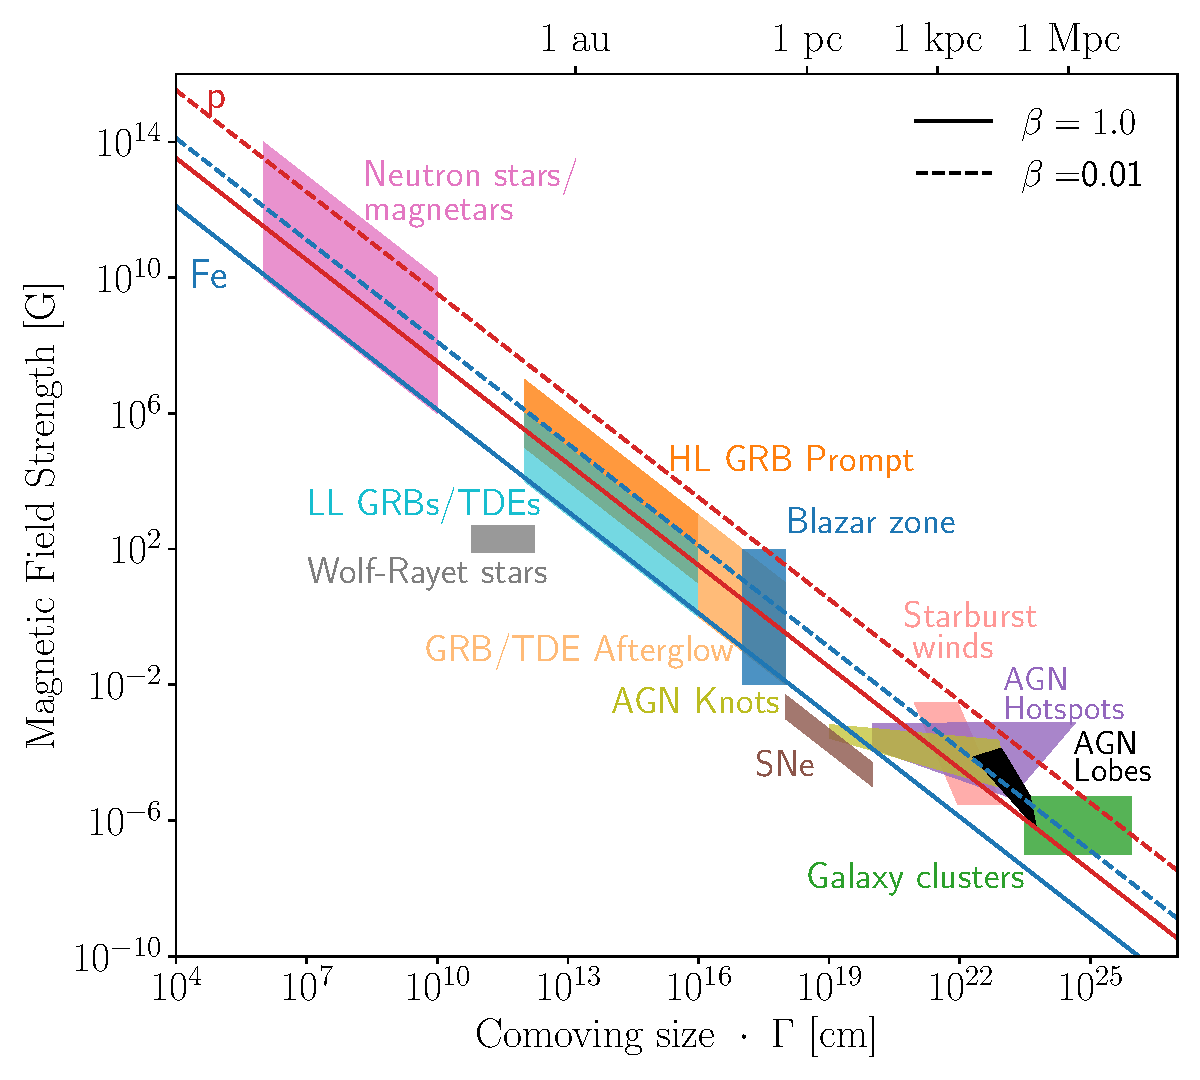
\includegraphics[width = 0.5\textwidth]{C:/Users/henri/OneDrive/Documents/NTNU/Semester 10/Masteroppgave/Plots/hillas.pdf}
    \caption{Hillas criterion for proton (blue line) and iron (red line) accelerated up to $10^{20}eV$ and $10^{21}eV$ respectively}
    \label{fig:hillas_c}
\end{figure}


\subsubsection{Macroscopic Acceleration mechanisms}
In order to accelerate particles to high energies, one needs to have a mechanism that can transfer energy to the particles. This usually happens through electromagnetic fields, and there are several ways this is thought to happen.

\textbf{One-shot acceleration}:
The simplest yet still a powerful way of accelerating particles is through what is called one-shot acceleration. In the presence of an ordered electricmagnetic fields, one can continuously accelerate charged particles which will follow the field lines. This can be induced from a rotating magnetic field or a straight electric field, all which create and electromagnetic force on a hypothetical charged particle. 
This could be the feature of some astrophysical objects such as neutron stars and black holes, usually in a quite close proximity to the object in question.% (ref cern paper)


\textbf{Second order Fermi acceleration/Diffusive acceleration}
In regions where one has high variability in the magnetic field strength, one can accelerate particles via scattering. The idea is that charged particles scatter on what can be seen as magnetic clouds and gain energy in the process due to the speed of the clouds. This mechanism is dubbed second order fermi acceleration due to the average energy gain of a particle being proportional to $(\frac{v}{c})^2$. Here $v$ is the speed of the cloud and $c$ is the speed of the particle. This is a slow process due to the proportionality to $v^2$, but as mentioned in \cite{Dermer_2001} can be a viable way of accelerating particles which already have a high energy. In modern times the magnetic mirrors that particles scatter on are thought to be plasma waves. The idea is that particles occupy a background magnetic field $B_0$ with a superimposed fluctuating electromagnetic field which arrise due to cold-plasma waves. The full formalism is described in \cite{BHradiation} at page 361. In trying to shorten the explination on only focuses on the resulting energy gain. The mean rate of change of the momentum of a particle is given as

\begin{equation}
    \left<\frac{dp}{dt}\right> = \frac{1}{p^2}\frac{\partial}{\partial p}\left[p^2D(p)\right] 
\end{equation}

where the real challenge lies in determining the diffusion coefficent $D(p)$ which is a function of the particle momentum and pitch angle. One will follow the approach found in \cite{O_Sullivan_2009} in which one only considers alfvén waves which take a one-dimensional power spectrum $W(k) \propto k^{-q}$, where $q$ is the spectral index and the total internal energy of the waves is given as $\frac{\delta B^2 }{8\pi}= \int_{k_{min}}^{k_{max}} W(k)dk$.   

As given in \cite{O_Sullivan_2009} the diffusion coefficient with current wave spectrum can be given as

\begin{equation}
    D(p) = \beta_a^2 \frac{\delta B^2}{B_0^2}\left(\frac{r_g}{\lambda_{max}}\right)^{q-1} \frac{p^2c^2}{r_g c}
\end{equation}

where $\beta_a = \frac{B}{\sqrt{4 \pi n_p m_p}c}$ is the alfvén speed, $r_g = \frac{pc}{ZeB}$ is the gyroradius of the particle, and $\lambda_{max}$ is the maximum wavelength of the waves, which will be specified when necessary, but if one is following \cite{O_Sullivan_2009} takes the value of $0.1 R$, i.e. a magnitude lower than the radius of the emitting region.

Form here one can estimate the acceleration timescale of a particle in a given region. The timescale is given as

\begin{equation}
    t_{acc} = \frac{p^2}{D(p)}
\end{equation}


\textbf{First order Fermi acceleration}
In regions where one has strong shock fronts, one can accelerate particles to high energies. These environments can be found several places where the interstellar medium is interacting with a powerful source of energy. One of the most famous examples of this is the supernova remnant where one sees a powerful shock front as a result of a supernova explosion.  
The first-order Fermi acceleration happens when particles traverse these strong shock fronts, and when a particle moves through the shock it gains energy proportional to $\frac{v}{c}$. In addition to this, there is a probability that the particle will stay in the accelerating region and 
experience several accelerations. 

In \cite{Dermer_2001} they can derive the relative power of a particle undergoing first-order Fermi acceleration in a relativistic shock, and it is given as 



\begin{equation}
    \dot p = \frac{2p}{t_u} = \frac{2cqB\Gamma}{mc^2 }
\end{equation}


where $t_u$ is the time in the upstream frame, $p$ is the momentum of the particle, $c$ is the speed of light, $q$ is the charge of the particle, $B$ is the magnetic field strength, $\Gamma$ is the Lorentz factor of the shock, and $m$ is the mass of the particle.

\textbf{Kink instabilities(KI) in jets}
Another method of acceleration which really is diffusive one shot acceleration related to AGN jets is acceleration via the kink instability in jets. The explanation of kink instability leading to acceleration is found in \cite{Alves_2018}. Kink instability is a hydrodynamic instability that arises in jets when the magnetic field is not aligned with the jet. If a perturbation is introduced to the jet, the resulting force on the jet structure will magnify the perturbation. This will lead the jet to a much more complicated structure, and twist the magnetic field lines. See figure \ref{fig:kink_instability} for an illustration. The paper argues that a highly tangled magnetic field and a large scale inductive electric field which is found throughout the kink-unstable region will lead to rapid energization of particles. 

\begin{figure}
    \centering
    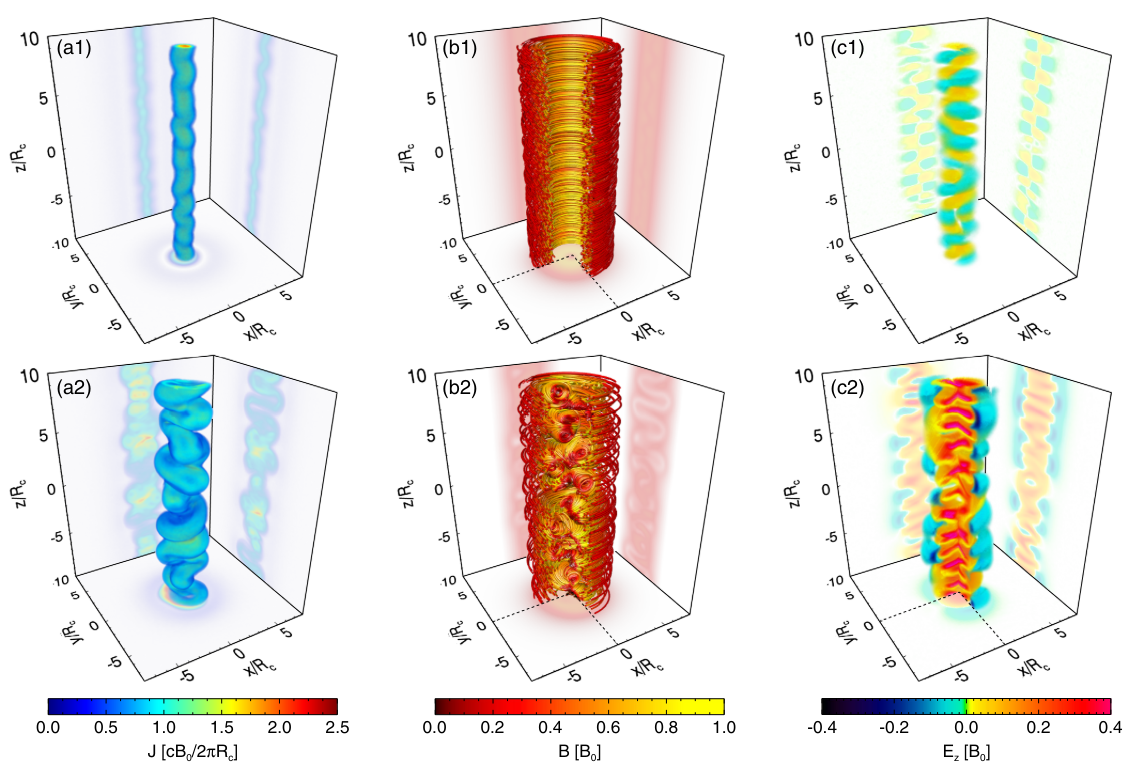
\includegraphics[width = 0.8\textwidth]{C:/Users/henri/OneDrive/Documents/NTNU/Semester 10/Masteroppgave/Plots/KI_instability.png}
    \caption{Simulations from \cite{Alves_2018} showing the evolution of kink instability in a jet. The upper panels shows the before the KI instability has been amplified, and the lower panel shows the jet after the instability has been amplified. From left to right the panels show, Current density, magnetic field lines, and axial electric field. }
    \label{fig:kink_instability}
\end{figure}

\subsection{UHECRs}

UHECRs are charged particles that are bombarding the Earth with energy exceeding 1 exaelectronvolt ($10^{18}$ eV) according to \cite{Alves_Batista_2019}. The exact origin of 
these particles is still a mystery but due to their high energies, they are thought to be extragalactic.
The composition of UHECRs ranges from protons to heavier nuclei such as helium or iron, and when these particles interact with the atmosphere they produce a shower of secondary particles.
The air showers can contain a lot of information such as energy and  direction, and through the use of large detectors, one can reconstruct the original cosmic ray and the spectra of UHECRs. In this section, I will discuss the nature of UHECRs, their energy loss mechanisms, and how they are detected.

%but due to the nature of UHECRs the location of their source is
%difficult to trace back to. This is because UHECRs are charged particles and therefore are deflected by the magnetic fields they encounter.

\subsubsection{Production and Energy loss}
The requirements to produce a UHECR are a charged particle and a powerful accelerator. During a particles acceleration and after it has escaped there are several ways a particle can lose energy.
In order to model them sufficiently one needs to take into account these energy loss mechanisms in their journey to Earth. 

The important parameters for this energy loss are its composition and its environment. In addition to energy, the interstellar magnetic field will also deflect the particles and therefore the direction of the particle will be changed during its propagation. 
What these effects can show us is that all UHECRs have a finite distance they can travel before they lose too much energy and therefore the volume in which they can be produced is limited.
Here I will briefly discuss the most important energy loss mechanisms.

\textbf{Photo-pair production}

\begin{equation}
    p + \gamma \rightarrow p + e^- + e^+
\end{equation}

For UHECRs, the most dominant sink of energy when under a certain energy threshold is the Bethe-Heitler process. In this process, a proton of sufficient energy interacts with the 
photon field in its vicinity and produces a pair of electrons and positrons. The photon field can vary from the cosmic microwave background to the generated field from different sources. 
The energy loss of this process is quite small $\sim \frac{2m_e}{m_p}= 10^{-3}$ of the original energy of the proton, but the process is very common, and therefore it is a significant energy loss over time.


\textbf{Photo-Pion production }
\begin{equation}
    p + \gamma \rightarrow \Delta^+ \rightarrow (p + \pi^0)\quad \text{or} \quad (\pi^+ + n)
    \label{eq:delta_resonance}
\end{equation}

Given enough energy the proton can interact with a photon field and produce a delta resonance. This resonance can then decay into a pion and a proton or a pion and a neutron. In this mechanism the original proton loses $m_p/m_\pi \approx 20\% $ of its energy resulting in a quite rapid loss of energy.This mechanisms is important since it also puts an upper limit on the UHECR energy for intergalactic particles. 
This limit, called the Greisen-Zatsepin-Kuzmin (GZK) limit comes from the UHECRs interacting with the cosmic microwave background in this delta resonance process. The limit caps proton energy at $5\times 10^{19}$ eV.


%\textbf{photodisintegration}
%mabye include this. 



%https://inspirehep.net/literature/1611251
% https://journals.aps.org/prl/abstract/10.1103/PhysRevLett.125.121106


\subsubsection{Detection}
When a high-energy cosmic ray hits the Earth's atmosphere, it sets off a cascade of interactions with air molecules, resulting in the emission of secondary particles and light. Detecting this cascade is much more feasible than capturing the original cosmic ray itself.

In addition, since the UHECR flux at high energy is extremely low ($<$1 particle per $\rm km^2$ per year for $E > 10^{19}$) one needs a large area to collect enough events. The largest UHECRs detectors of present are the Pierre Auger Observatory and the Telescope Array.

The Pierre Auger Observatory is located in Argentina and is the largest detector of its kind. It consists of 1660 Cherenkov detectors spread over 3000 km$^2$ and 27 fluorescence telescopes in four locations. With these instruments, the observatory is very capable of reconstructing the air showers and therefore the energy and direction of the cosmic ray. The observatory has a blind spot in the night sky and therefore the observatory is complemented by the Telescope Array located in Utah. The Telescope Array is a smaller observatory with 507 scintillator detectors and 3 fluorescence telescopes. Combined they have been able to map the full sky of UHECRs.

When a cosmic ray interacts with the atmosphere it produces a shower of secondary particles. These particles will then interact with several of the Cherenkov detectors located on the ground at approximately the same time. By measuring the time difference between the detectors one can reconstruct the direction of the cosmic ray. The energy of the cosmic ray can also be reconstructed by combining the measurements from the Cherenkov detectors. There is also a secondary detector in the Pierre Auger Observatory called the fluorescence detector. This detector will make use of the very faint glow that the air shower produces when it interacts with particles in the atmosphere. The detector will then observe a shower as a trace of light in the sky and by measuring the total amount of light one can infer the energy, while the shape of the trace can give naturally the direction of the cosmic ray.

\subsubsection{Emissivity estimates}
\label{sec:emmisivity}
From the detectors on earth great strides have been made in modeling the flux of UHECRs. The flux is modeled as a power law and the model parameters are taken from \cite{thepierreaugercollaboration2017pierre} and are shown in table \ref{tab:UHECR_flux}. The flux is tohught to be separated into contributions from extragalactic sources and galactic sources, and with this information one can start to make tangible estimates of the sources of UHECRs.
One such estimate is the emissivity of UHECR sources. The emissivity is a measure of the energy released per unit time per unit volume. The question one can ask is what is the necessary emissivity of UHECRs to explain the observed flux here on Earth? In other words, what is the required energy injection rate per unit volume of UHECRs?


\begin{figure}
    \centering
    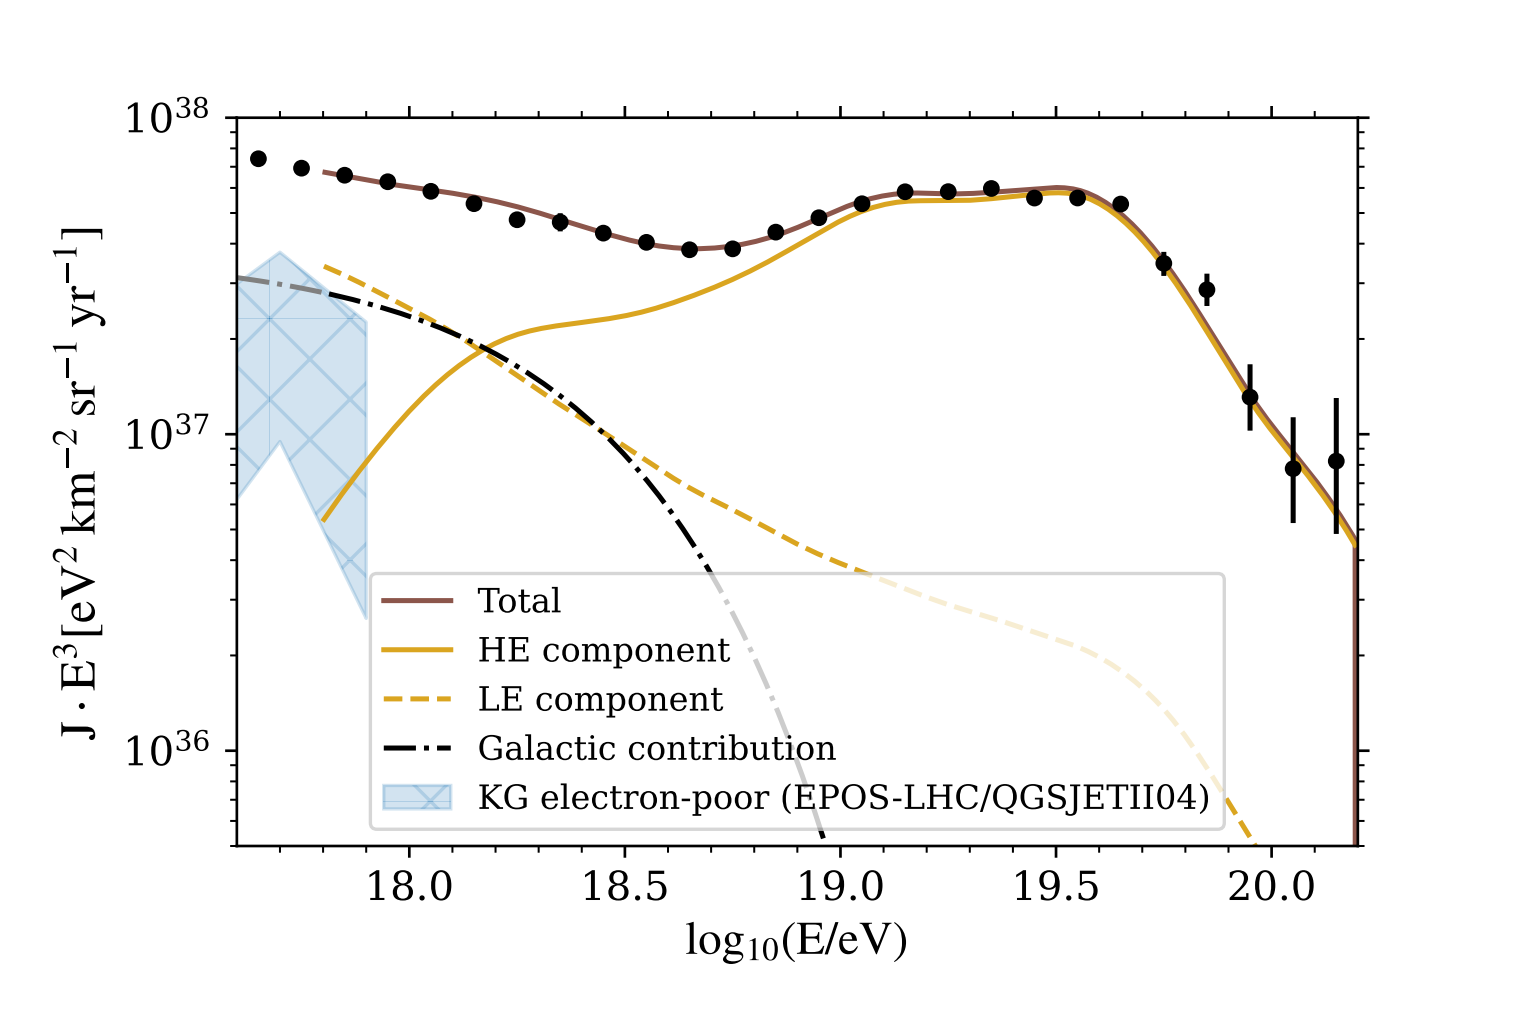
\includegraphics[width = 0.7\textwidth]{C:/Users/henri/OneDrive/Documents/NTNU/Semester 10/Masteroppgave/Plots/UHECRs.png}
    \caption{The diffuse flux of UHECRs as measured by the Pierre Auger Observatory and the Telescope Array. The flux is separated into galactic and extra galactic sources where the total spectrum follows the black dots. Image taken from \cite{Abdul_Halim_2023}}
    \label{fig:flux_UHECRs}
\end{figure}



\begin{equation}
    J(E_v) = \begin{cases} 
        J_0 \left(\frac{E_v}{E_{\text{ank}}}\right)^{-\gamma_1}  \text{if } E_v < E_{\text{ank}} \\
        J_0 \left(\frac{E_v}{E_{\text{ank}}}\right)^{-\gamma_2} \left(1 + \left(\frac{E_{\text{ank}}}{E_s}\right)^{\gamma_d}\right) \left(1 + \left(\frac{E_v}{E_s}\right)^{\gamma_d}\right)^{-1}   \text{if } E_v \geq E_{\text{ank}}
    \end{cases}
\end{equation}

\begin{table}
    \centering
    \begin{tabular}{|c|c|c|c|c|c|}
        \hline
        $J_0$ & $E_{\text{ank}}$ & $\gamma_1$ & $\gamma_2$ &$\gamma_d$& $E_s$\\
        \hline
        $3.3 \times 10^{-19} $ & $4.82\times 10^{18}$ & 3.14  & 4.2 & 3.14& $4.2 \times 10^{19}$  \\
        \hline
    \end{tabular}
    \caption{The model parameters for the astrophysical flux of UHECRs as measured by the Pierre Auger Observatory and the Telescope Array.}
    \label{tab:UHECR_flux}
\end{table}




By separating the flux into contributions from extragalactic sources and galactic sources one can estimate the observed energy density in the Universe of extragalactic UHECRs $u_{\rm UHECR}$. Subsequently, one can define an energy loss time for a UHECR as the loss length divided by the speed of light $c$.
The loss length is a measure of the distance a UHECR can travel before its energy drops below a certain threshold, and for our simple analysis, we will use the length of $1 Gpc$. This number is comparable in magnitude as found by \cite{Stanev_2009}, but as the loss length is dependent on initial energy and composition our number will be an approximation.

The emissivity of UHECRs is then given as

\begin{equation}
    \epsilon_{\rm UHECR} = \frac{u_{\rm UHECR}}{t_{\rm loss}} = \frac{u_{\rm UHECR}}{D_{\rm loss}/c} = \frac{4\pi c \int_{E_0}^{E_{\rm max}}J_{\rm extragalactic}(E)E dE}{c D_{\rm loss}} %\approx 9\times 10^{44} \frac{\rm erg}{\rm Mpc^3 \rm yr}.
\end{equation}

Here $u_{UHECR}$ represents the energy density of extragalactic UHECRs, $t_{loss}$ is the energy loss time, $D_{loss}$ is the loss distance, $J(E)$ is the flux of UHECRs, $E_0 = 1$ exaelectronvolt, is the minimum energy of the flux where extragalactic UHECRs become important, and $E_{max}$ is the maximum energy of extragalactic UHECRs.
By using the paramter value in table \ref{tab:UHECR_flux} for the UHECRs flux one recives the value of $9 \times  10^{44} \frac{\rm erg}{\rm Mpc^3 \rm yr}$ for the emissivity of UHECRs.
This emissivity is a crude estimation of the required energy injection rate of UHECRs and is meant to give a rough estimate. This is comparable to a more thorough analysis from \cite{PhysRevLett.125.121106} which received a value of $6 \times 10^{44} \frac{\rm erg}{\rm Mpc^3 \rm yr}$.




\subsection{Neutrinos}

The second particle of interest is the neutrino. Neutrinos compared to UHECRs are neutral particles that are produced in various processes in the Universe.
The most common and well-known is the fusion reaction in the sun where neutrinos are produced in the pp chain. On the other hand the neutrinos of focus in this paper 
are high-energy neutrinos that are likely produced in the same sources as the UHECRs.



\subsubsection{Production and Energy loss}
The production sites of high-energy neutrinos is not clear, but they are thought to be produced in the same sources as UHECRs 
and in this section, I will go through the most probable way of producing high-energy neutrinos in sources such as AGN.

\textbf{Hadronic processes}:

Hadronic processes can release neutrinos with sufficiently high energy to explain the observations here on Earth. 
Processes such as nuclear interactions are limited by the binding energy of the nucleus and accelerating a neutrino after its production is difficult.
Therefore, a common way of producing the observed neutrinos is through the decay of pions. The most important decay is the decay of charged pions into muons and muon neutrinos as seen in equation \ref{eq:pion_decay}


\begin{equation}
    \pi^+ \rightarrow \mu^+ + \nu_\mu \rightarrow e^+ + \nu_e + \nu_\mu + \bar{\nu_\mu}
    \label{eq:pion_decay}
\end{equation}

I will discuss two possible ways of producing these pions in two different environments. 


In a proton-rich environment where the protons can accelerate up to high energies, one can produce pions through the following process
\begin{equation}
    p + p \rightarrow \begin{cases}
        \pi^+ + n+ p \\
        \pi^- + \pi^+ +p + p  \\
        \pi^0 + p+p
    \end{cases}
\end{equation}

The energy of these protons above a few GeV is enough to introduce the delta-baryon resonance, but usually one does not have a proton rich environment.
Therefore, the most efficient way of producing pions is through the already seen delta resonance when a proton interacts with a photon, this is seen in equation \ref{eq:delta_resonance}.
This process being the cooling process of UHECRs is interesting and indicates that a source that produces high energy neutrinos likely is inhabited by very energetic charged particles. 

After having produced the neutrinos it also becomes important to understand their behavior during their travel to Earth. Here I will highlight two points


\textbf{Neutrino oscillations}:
In the previous paragraph, I discussed the production of these neutrinos, but not their initial flavor.
The pion decay model is known to produce a flavor composition of $\nu_e : \nu_\mu : \nu_\tau = 1:2:0$. 
A naive thought would be an identical composition observed on Earth, but sadly this is not the case. 
The reason for this is that the neutrinos' mass state can oscillate between the different flavors. Therefore, the neutrinos produced in the source will oscillate during their travel to Earth and when they reach us one would expect a 
uniform mix of the three flavors, $ \nu_e: \nu_\mu: \nu_\tau = 1:1:1$.

\textbf{Energy loss}:
To model the travel of a neutrino of any flavor one only needs to take into account the interaction of the neutrino with the expanding universe. Since it is so weakly interacting the only 
source of energy loss the flux of neutrinos will experience is the redshift created by the expansion of the Universe. This redshift is the same as the one discussed in the previous section and the neutrinos 
behave the same way light does in this manner with a drop in energy proportional to $(1+z)$.



 

\subsubsection{Detection}
\begin{figure}
    \centering
    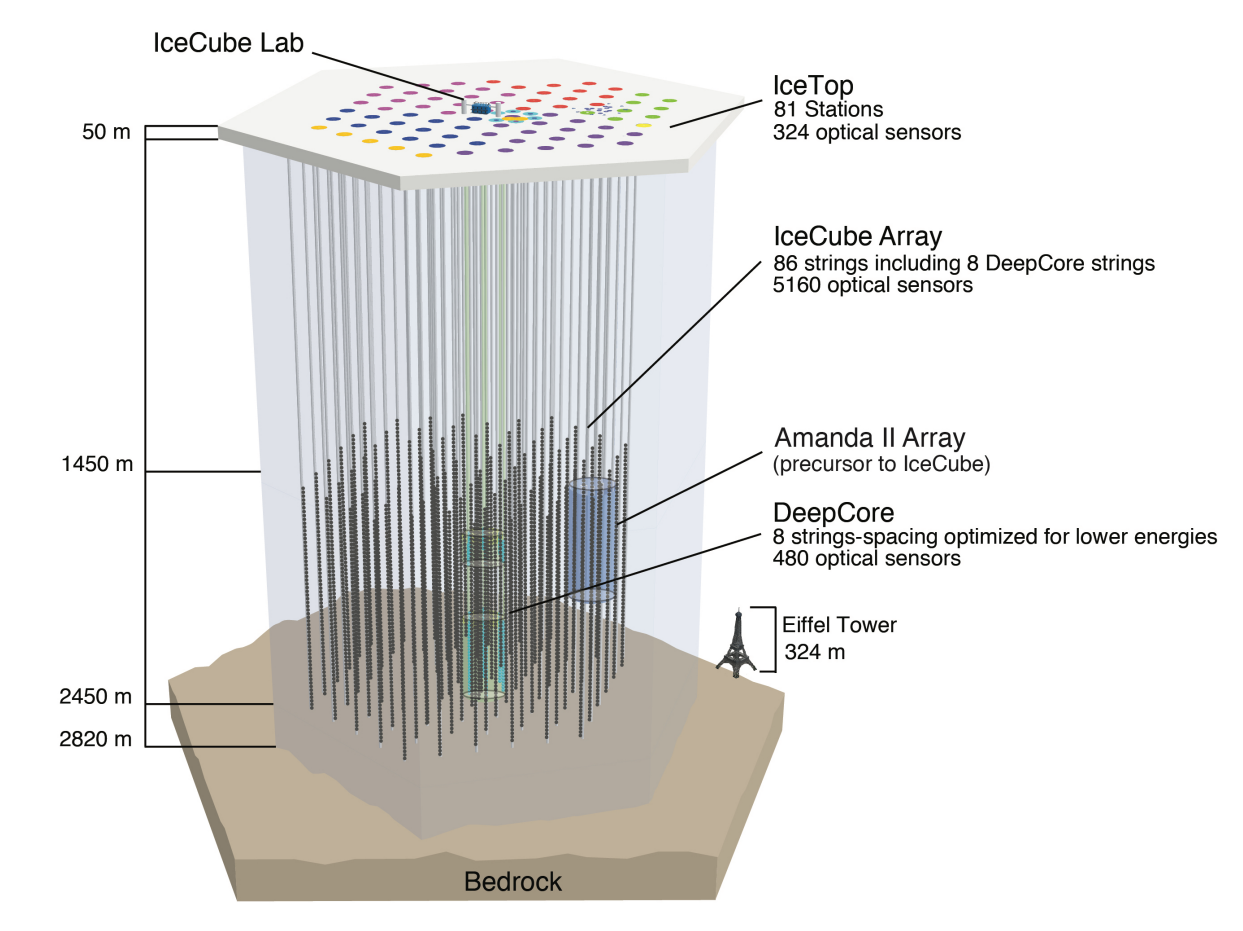
\includegraphics[width = 0.5\textwidth]{C:/Users/henri/OneDrive/Documents/NTNU/Semester 10/Masteroppgave/Plots/Ice_cube_layot.png}
    \caption{The IceCube neutrino observatory. The detector is located at the South Pole and is a large block of ice instrumented with photomultiplier tubes. Image taken from \cite{Andeen_2019}}
    \label{fig:Ice_cube}
\end{figure}

Neutrinos are weakly interacting matter particles and therefore are very difficult to detect. This makes them excellent candidates for the study of the Universe since they can travel large distances without interacting, but make them 
quite difficult to detect with high accuracy. The most famous detector and the one used in this paper is the IceCube neutrino observatory. This detector is precisely what it sounds. It is a large block of ice with a size equal to a cubic kilometer located at the South Pole.
The observatory uses the ice located deep in the South Pole as a giant Cherenkov detector. The ice is instrumented with photomultiplier tubes that can detect the Cherenkov radiation produced by neutrinos interacting with the ice. 
More precisely the observatory is fitted with 5160 photomultiplier tubes located at a depth of 1450-2450 m. The photomultipliers are divided into 86 strings of 60 modules each. The detector is also complemented by the DeepCore detector which is a denser array of photomultiplier tubes located in the center of the detector. See Figure \ref{fig:Ice_cube} for a visual representation of the detector.
The energy range for this detector is from 10 GeV to 10 EeV. The interaction of neutrinos with the water molecules in the ice can produce charged leptons (muons, electrons or taus). These charged particles if energetic enough will then produce Cherenkov radiation which can be detected by the photomultiplier tubes.

\begin{figure}
    \centering
    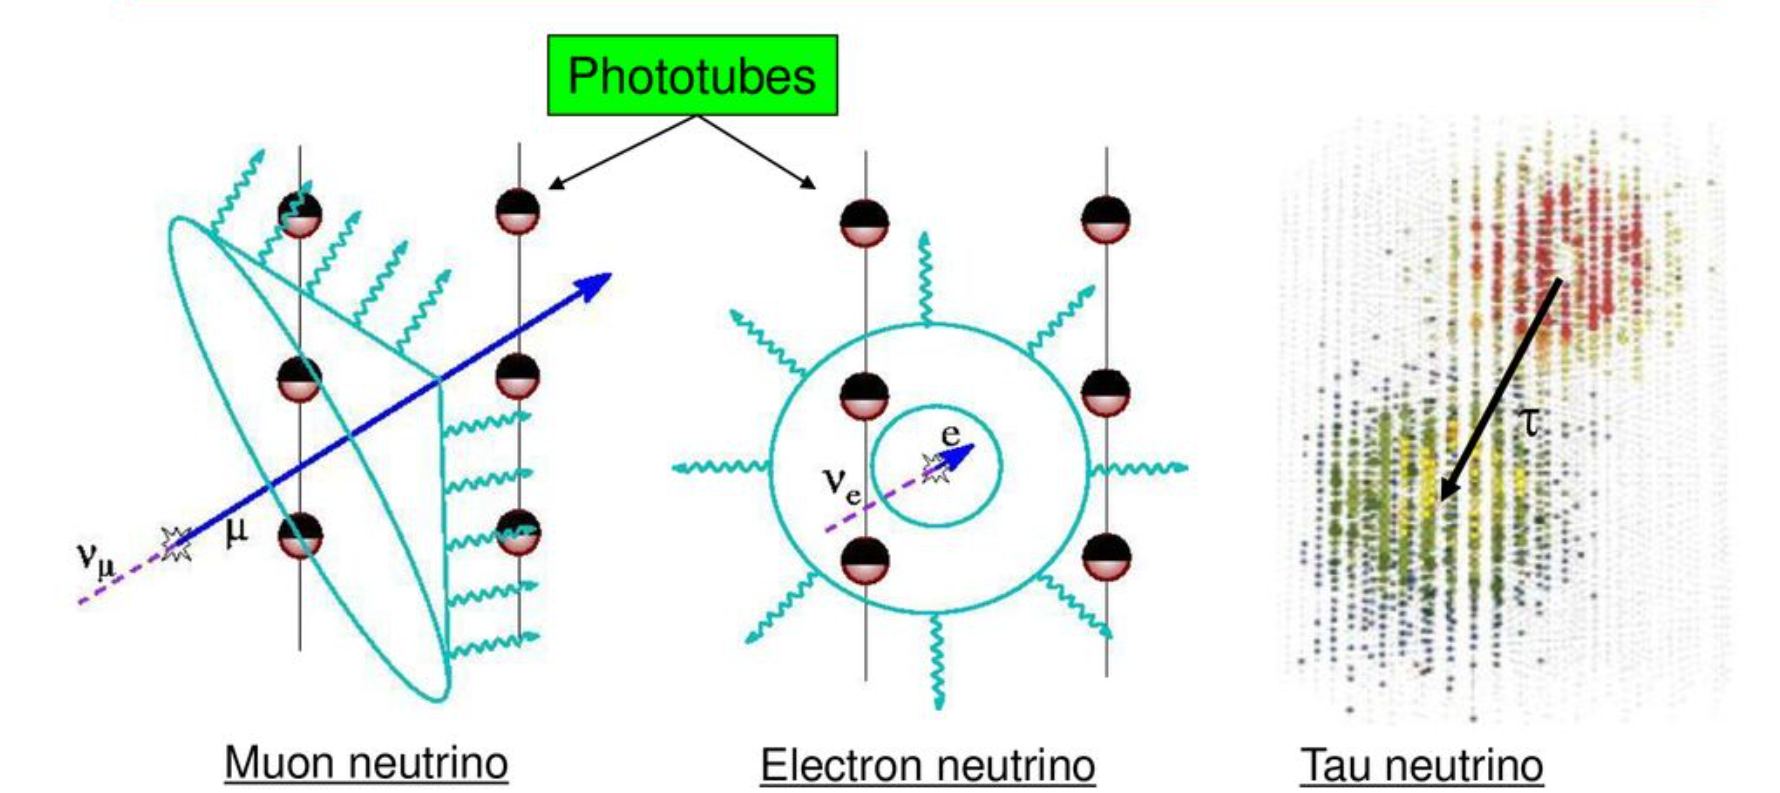
\includegraphics[width = 0.7\textwidth]{C:/Users/henri/OneDrive/Documents/NTNU/Semester 10/Masteroppgave/Plots/Track_events_neut.png}
    \caption{The difference between track and cascade events in the IceCube detector. The left image shows a track event where a muon has traveled through the detector. The middle image shows a cascade event where a neutrino has interacted with the ice and produced a shower of particles. The right image shows a double bang event where a tau neutrino has produced a tau lepton which has then decayed. Image taken from \cite{LectureA}}
    \label{fig:track_neut}
\end{figure}

The detection of neutrinos in IceCube are seperated into categories which often relates to the flavour of neutrino being detected. In figure \ref{fig:track_neut} one can see the distinct signature left by different flavour neutrinoes. The different signatures mean that for estimating arrival direction only track events can be used, which is caused by mostly muon neutrinos. Track events have the disadvantage of being worse for estimating the energy of the neutrino, due to part of the interaction happening outside the detector. On the other hand cascade and double bang events are better for estimating the energy of the neutrino, but are worse for estimating the direction of the neutrino.


\subsubsection{Emissivity estimates}
\label{sec:emmisivity_neutrinos}

Armed with the required knowledge above one can also make simple arguments for the sources of these neutrinos based on the observed 
flux here on Earth. The flux used in this paper is the diffuse flux of neutrinos as measured by the Ice Cube observatory. The flux is shown in figure \ref{fig:flux_neutrinos}. 
For any calculations, we use the astrophysical flux as modeled as a power law. The power law is of the form 

\begin{equation}
    \Phi(E) = \Phi_0 \left(\frac{E}{E_0}\right)^{-\gamma}
\end{equation}

with $\Phi_0$ being the normalization constant, $E_0$ being the reference energy and $\gamma$ being the spectral index. The model parameters are seen in table \ref{tab:neutrino_flux} and taken from \cite{Abbasi_2022}.

\begin{table}
    \centering
    \begin{tabular}{|c|c|c|}
        \hline
        $\Phi_0$ & $E_0$ & $\gamma$ \\
        \hline
        $6.7\times 10^{-18} GeV^{-1} cm^{-2} s^{-1} sr^{-1}$ & $100 TeV$ & 2.37 \\
        \hline
    \end{tabular}
    \caption{The model parameters for the astrophysical flux of neutrinos as measured by the Ice Cube observatory.}
    \label{tab:neutrino_flux}
\end{table}

The emissivity of neutrinos is calculated in the same way as for UHECRs. The only difference is the loss time. Neutrinos do not lose energy in the same way as UHECRs and therefore the loss distance will be the size of the Universe. 
The modeled emissivity is then approximately $1.54 \times 10^{44} \rm erg/Mpc^3/yr$. 

\begin{figure}
    \centering
    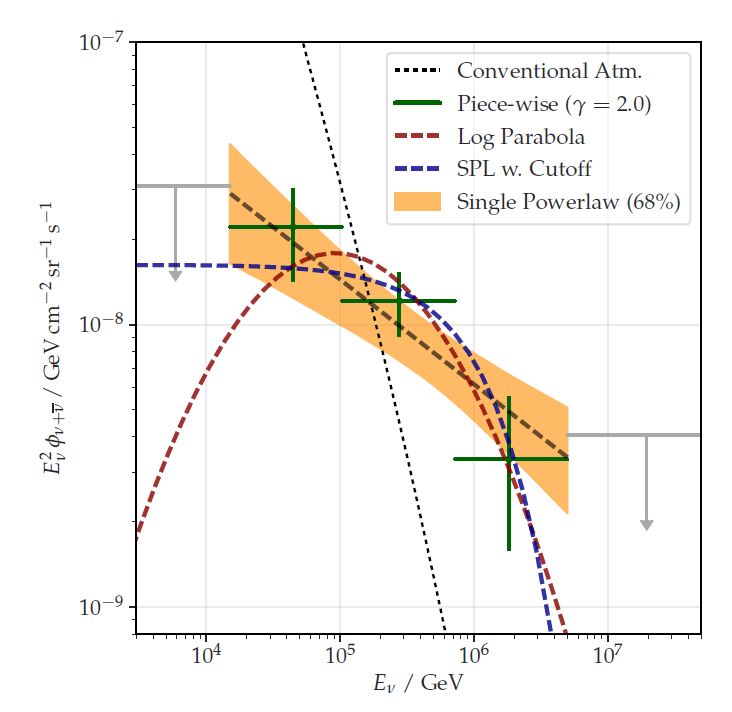
\includegraphics[width=\textwidth]{C:/Users/henri/OneDrive/Documents/NTNU/Semester 10/Masteroppgave/Plots/Ice_cube_flux_astro.png}
    \caption{The diffuse flux of neutrinos as measured by the Ice Cube observatory. The y-axis on the left image is the number of events per bin.  The flux is separated into contributions from atmospheric neutrinos and astrophysical neutrinos. The right image is the model astrophysical flux as measured by ICE CUBE. Images taken from \cite{Abbasi_2022} }
    \label{fig:flux_neutrinos}
\end{figure}